\documentclass[10pt,a4paper]{article}
%\documentclass[10pt,a4paper,twoside]{article}
\usepackage{a4wide}
\linespread{1.359140914229522617680} 
\usepackage[utf8]{inputenc}
\usepackage[T1]{fontenc}
\usepackage[german]{babel}
\usepackage{amssymb}
\usepackage{graphicx}
\usepackage{url}

\newcommand{\degree}{$^\circ$}

\author{Michael F. Schönitzer}
\title{Der Kosmische Mikrowellenhintergrund und seine Anisotropien}


\begin{document}
\maketitle

\section{Die Vorhersage und Entdeckung des Kosmischen Mikrowellenhintergrunds}
Albert Einstein und Willem de Sitter beschrieben 1917 zum ersten Mal das Universum als Ganzes mit dem Formalismus der allgemeinen Relativitätstheorie unter der Annahme eines isotropen, homogenen und statischen Universums.
Nachdem Edwin Hubble 1925-29 entdeckt hatte, dass sich alle Galaxien scheinbar von uns weg bewegen und diese Bewegung umso schneller ist, je weiter die Galaxie von uns entfernt sind, stellte Georges Lemaître 1927 fest, dass die Annahme eines statischen Universum nicht notwendig richtig sei, sondern dass das Universum expandiert. Lemaître war auch der erste, der aus der Expansion des Universums darauf schloss, dass es dann in der Vergangenheit einen Zeitpunkt gegeben haben müsse, zu welchem das Universum punktförming war -- die Urknall-Theorie war geboren.
Die Expansion kann durch die von Alexander Friedmann bereits 1922 aufgestellten Friedmann-Gleichungen beschrieben werden.
Der Unterschied zwischen Einsteins und Friedmanns Modell, war dass Einstein die sogenannte kosmologische Konstante in sein Modell einführte und ihre Größe derart bestimmte, dass die Gleichungen ein statisches Universum beschrieben. Friedmann verwarf die unbegründete Annahme des statischen Universums und setze die Konstante gleich Null.
Heute wissen wir, dass das Universum zwar nicht statisch ist sondern sich seit dem Urknall ausdehnt, die Kosmologische Konstante jedoch trotzdem nicht Null ist.
Die physikalische Interpretation der Kosmologischen Konstante entzieht sich bisher unserem Wissen, man bezeichnet sie heute oft verallgemeinert als Dunkle Energie.

Die aus der allgemeinen Relativitätstheorie folgende allgemeine Beschreibung des Universums hängt von einer Reihe von Parametern ab, welche entscheiden, ob das Universum expandiert oder sich zusammenzieht und ob es flach oder gekrümmt ist. Diese zu bestimmen, gehörte über lange Zeit zu den wichtigen Aufgaben der Kosmologie. Inzwischen kennen wir sie genau genug, um sagen zu können, dass wir in einem flachen, seit dem Urknall expandierendem und dabei abkühlendem Universum leben.

In den 1940ern folgerten George Gamow, Ralph Alpher und Robert Herman aus der Urknalltheorie, dass es einen Strahlungshintergrund in Mikrowellenbereich geben müsste\cite{S+W00}:

Kurz nach dem Urknall entstanden im Universum eine Vielzahl an Elementarteilchen, welche mit der Strahlung im thermischen Gleichgewicht standen. Mit der Zeit sank durch die Expansion des Universums die Dichte und damit auch die Temperatur des Strahlungs-Materie-Gemischs immer weiter ab, bis nach etwa 380.000 Jahren die Temperatur auf etwa 3.000\ Kelvin gesunken war und sich somit die Protonen und Elektronen zu Wasserstoffatomen verbinden konnten.
Man spricht hier -- nicht ganz richtig -- von Rekombination. Nach dieser nahezu schlagartigen Rekombination, gab es keine freien Elektronen mehr, wodurch die Photonen nicht mehr durch Thomson-Streuung abgelenkt wurden und von nun an frei durch das Universum liefen. Das Universum wurde sozusagen schlagartig durchsichtig. Die Photonen von damals durchfliegen das Universum bis heute. Ihre Frequenzverteilung entspricht der eines Schwarzkörpers, da sie vor der Rekombination mit der Materie im thermischen Gleichgewicht standen. Ihre Temperatur entsprach der des Gleichgewichts, wurde jedoch seither durch die kosmische Expansion stark rotverschoben ($z\approx 1.000$). Die Temperatur der Kosmischen Hintergrundstrahlung (englisch cosmic microwave background, kurz CMB) beträgt heute etwa 2,7 Kelvin.\cite{Schneider}

Nach der erfolglosen Suche zahlreicher astrophysikalischer Teams entdeckten 1964 Arno Penzias und Robert Woodrow Wilson zufällig den Mirkrowellenhintergrund, als sie an einer neuen empfindlichen Antenne arbeiteten und ein Störsignal fanden, dass stets gleich war, unabhängig davon, in welche Richtung die Antenne ausgerichtet war. Nachdem das Signal auch nicht durch Reinigung der Antennen verschwand und sie keine Erklärung dafür fanden, wandten sie sich an andere Physiker. Die Kosmologen um Robert Dicke in Princeton identifizierten das Signal schließlich als kosmische Hintergrundstrahlung.\cite{S+W00} Der Fund des CMB gilt als eine der wichtigsten Entdeckungen der Kosmologie und als Bestätigung des Urknallmodels. Untermauert wird dies dadurch, dass das Spektrum äußerst präzise einem Schwarzkörper-Spektrum entspricht und über den gesamten Himmel äußerst gleichmäßig ist, was zeigt, dass es sich dabei nicht um eine Überlagerung von vielen kleinen Stahlungsquellen handelt.

\begin{figure}
\center
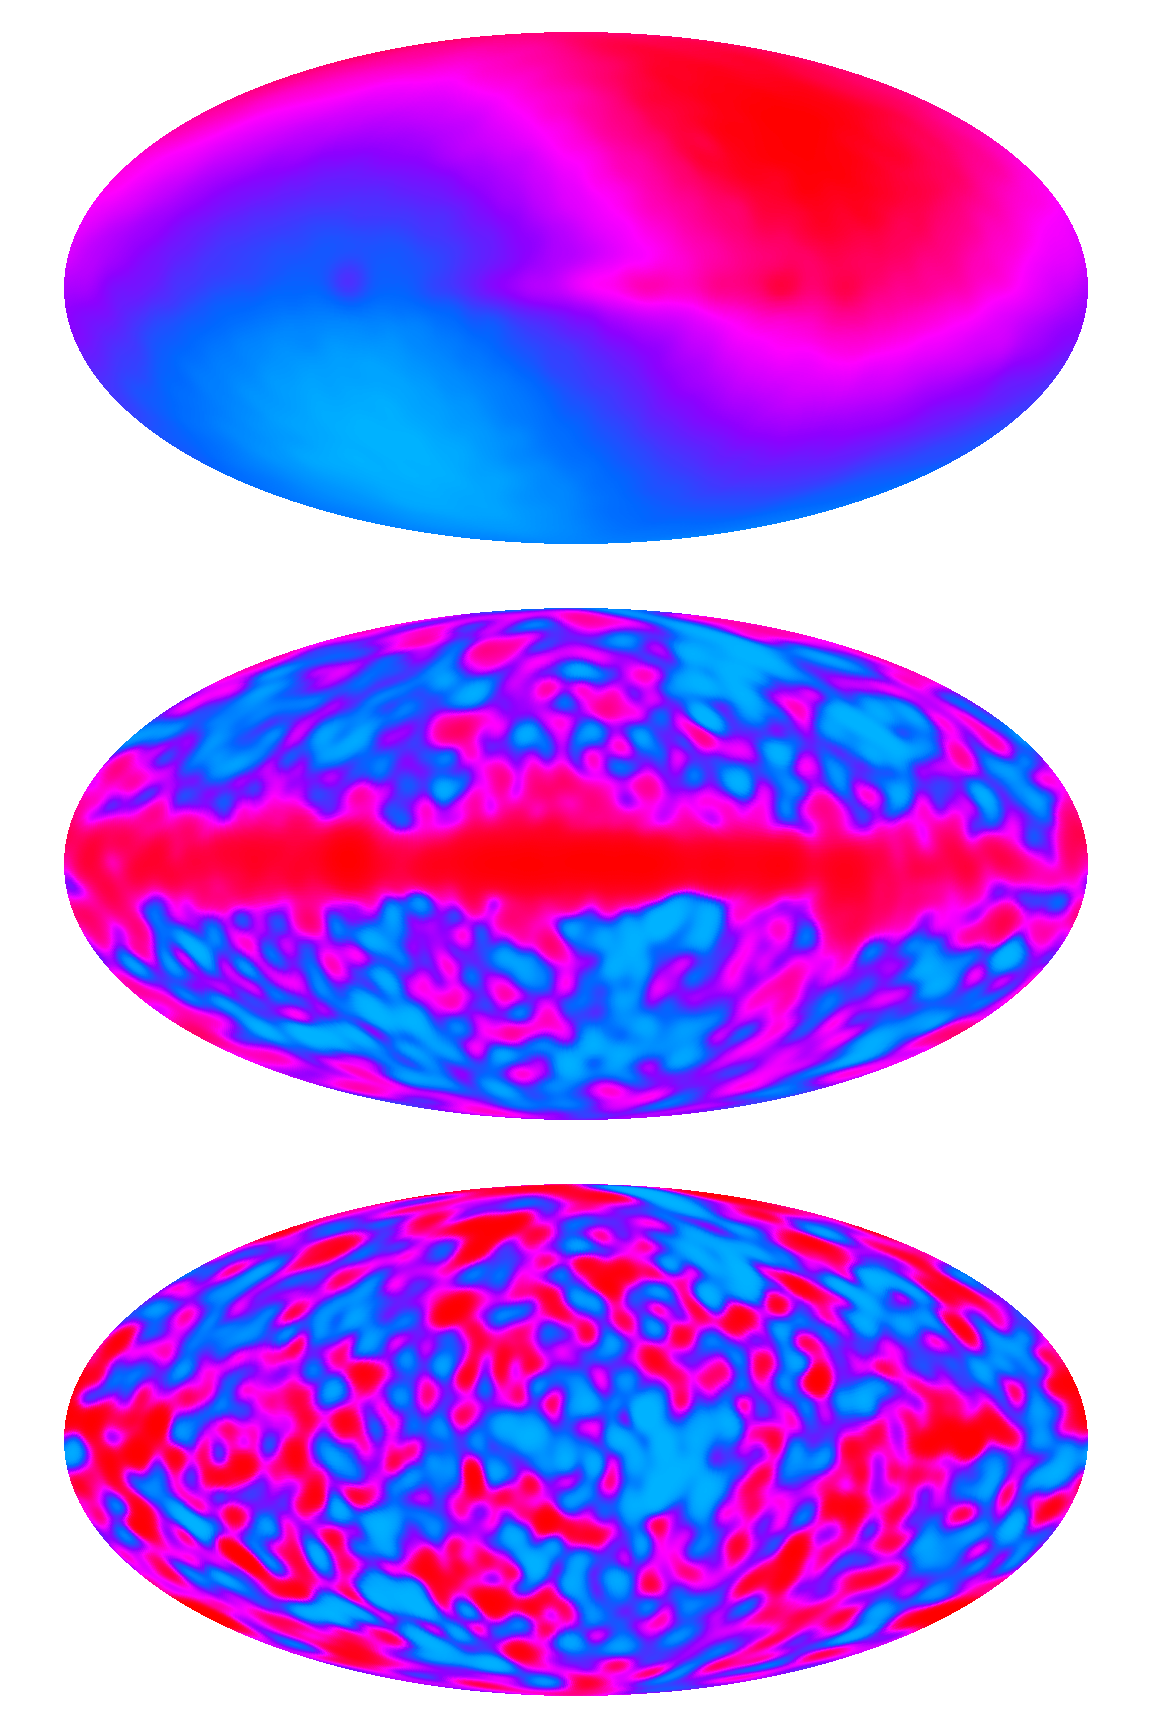
\includegraphics[scale=0.15]{COBE_cmb_2}
\caption{Die von COBE gemessenen Temperaturfluktuationen. Oben erkennt man nur die Dipolabweichung von der Größe $10^{-3}$. Entfernt man diese erkennt man die Anisotropien mit Überlagerungen. Bei der untersten Abbildung wurden die Vordergrundobjekte entfernt. } %Wort Dipolabweichung
\label{cobe}
\end{figure}

Die extreme Isotropie der Strahlung stellte jedoch auch ein Problem dar. Die heutigen Strukturen im Universum können sich nur gebildet haben, wenn auch im frühen Universum vor der Rekombination bereits Dichteschwankungen existiert haben. Diese müssten sich jedoch in Schwankungen in der Temperatur des CMB niedergeschlagen haben. Man begann also direkt nach der Entdeckung der Hintergrundstahlung damit, Anisotropien in ihr zu suchen. Von 1965 bis 1992, also fast drei Jahrzehnte lang, blieb diese Suche erfolglos.\footnote{Mit Ausnahme einer Dipolabweichung, welche dadurch erklärt werden kann, dass sich die Erde im Bezug auf den CMB bewegt. Dadurch kommt es zu einer Dopplerverschiebung von $10^{-3}$\%} %Wort Dipolabweichung
In dieser Zeit wurden sowohl durch theoretische Vorhersagen als auch durch die experimentellen Befunde (nämlich keine) die Vorhersagen der Stärke der Temperaturschwankungen von 10\% auf 0,001\%  herunter korrigiert.\cite{S+W00}
Die theoretische Grundlage dahinter ist, dass man inzwischen erkannte, dass nicht die gewöhnliche, sogenannte baryonische Materie, sondern die Dunkle Materie im Universum vorherrscht.
Als gerade ernste Zweifel an der Richtigkeit der Theorien aufkam, brachte der Satellit COBE den Durchbruch. Dieser konnte nicht nur bestätigen, dass das Spektrum extrem genau dem eines Schwarzkörpers entspricht, %dopplung
er fand auch die lange gesuchten Anisotropien.

Da man -- wie wir in den beiden folgenden Kapiteln sehen werden -- aus den Anisotropien des CMB viele wichtige Informationen gewinnen kann, insbesondere die oben angesprochenen Parameter der Beschreibung des Universums, wurden seitdem etliche Experimente zur genaueren Vermessung der Schwankungen unternommen. Wir werden sie in Kapitel \ref{Missionen} ansprechen.

\section{Die Ursachen der Anisotropien}
Bei den Ursachen der Schwankungen im CMB unterscheidet man zwischen primären und sekundären Anisotropien. Die primären Anisotropien sind die Effekte, die zum Zeitpunkt der Entstehung des CMB ihren Ursprung haben, während die sekundären Anisotropien erst später auf dem Weg der Photonen durch das Universum entstanden.

Die wichtigsten Effekte der primären Anisotropien sind:
\begin{itemize}
\item Photonen aus Gebieten mit einer höheren Massendichte mussten aus dem Gravitationspotentialtopf entkommen, dabei verloren sie einen Teil ihrer Energie, was einer Rotverschiebung entspricht. Photonen aus Gebieten niedrigerer Masse bekommen hingegen Energie vom Potential und werden ins Blaue verschoben. Andererseits wird dieser Effekt dadurch teilweise kompensiert, dass die Gravitation zu einer Zeitdilatation führt. Daher stammen die Photonen der dichteren Regionen aus einer ein kleines bisschen früheren Zeit, zu welcher das Universum noch heißer war. Beide Effekte werden zusammen als Sachs-Wolfe-Effekt beschrieben.\cite{Schneider} %bezeichnet?
\item Die Dichteschwankungen im frühen Universum führen zu Geschwindigkeiten der Materie -- zusätzlich zur Geschwindigkeit der Expansion des Raumes (Pekuliargeschwindigkeit genannt). Die Elektronen, mit denen die Photonen das letzte Mal streuen, haben also eine von der Dichte abhängige zusätzliche Geschwindigkeitskomponente.\cite{Schneider} %mehr?
\item Wird in einem kleinem Gebiet die Baryonendichte erhöht, werden die Baryonen adiabatisch komprimiert und dadurch heißer. Da die Baryonen mit den Photonen im thermischen Gleichgewicht stehen werden somit auch die Photonen energiereicher.\cite{Schneider}
\end{itemize}

Zu den sekundären Anisotropien gehören insbesondere:
\begin{itemize}
\item Wir wissen heute, dass es zwischen dem Zeitpunkt der Rekombination und heute eine Re\-ionisation gegeben haben muss. Daher gibt es bis heute freie Elektronen im Universum, an welchen die Photonen streuen können. Da die Thomson-Streuung weitgehend isotrop ist, ist die Richtung des Photons nach der Streuung weitgehend unabhängig von seiner Richtung vor der Streuung. Die gestreuten Photonen tragen keine Information über die Fluktuationen des CMB mehr. Dadurch werden die Anisotropien um den Faktor geschwächt, um den die Photonen eine Streuung erfahren.\cite{Schneider}
\item Auf dem Weg zu uns durchlaufen die Photonen des CMB ein Universum, in welchem sich die anfangs kleinen Dichteschwankungen zu immer ausgeprägteren Strukturen entwickeln. Dabei durchlaufen sie eine Vielzahl von Potentialtöpfen. Beim durchqueren eines Potentialtopfes werden die Photonen analog zum Sachs-Wolfe-Effekt zunächst blau- und dann wieder rotverschoben. Das Durchlaufen eines Potentialtopfs mit gleich hohen Seiten verändert die Energie nicht. Über die kosmische Entfernungen gemittelt ist dies genau dann der Fall, wenn das Gravitationspotential im Universum insgesamt zeitlich konstant ist. Man kann zeigen, dass dies nur in einem Universum nach dem Einstein-de-Sitter-Modell der Fall ist -- in allen anderen kosmologischen Modellen kommt es zu einer Veränderung der Frequenzen der CMB-Photonen. Man nennt dies den Integrierten Sachs-Wolfe-Effekt.\cite{Schneider}
\item Außerdem werden die Photonen beim Durchlaufen des Gravitationspotentials der kosmischen Strukturen abgelenkt. Der Winkel, unter welchem wir Photonen des CMB beobachten, entspricht also nicht genau ihrer Position zum Zeitpunkt der Rekombination -- dadurch werden die Anisotropien auf kleinen Winkelskalen verschmiert.\cite{Schneider}
\item An den Elektronen des heißen Gases von Galaxienhaufen können Photonen streuen. %was zu richtung sagen? (schneeider 253)
Durch die Streuung ändert sich die Energie der Photonen ein wenig: sie haben nach der Compton-Streuung im Mittel eine höhere Frequenz. Dadurch wird die Zahl der hochfrequenten Photonen relativ zum Planckspektrum erhöht, während die Zahl der niederfrequenten Photonen erniedrigt wird. Dies nennt man den Sunjajew-Seldowitsch-Effekt (englische Transkription: Sunyaev-Zeldovich-Effekt), man kann ihn in den CMB-Daten erkennen, wenn man über ein breites Frequenzband misst. Man kann ihn damit einerseits aus den Daten herausrechnen, andererseits kann man ihn verwenden, um Galaxiehaufen zu finden und ihre Gastemperatur und -dichte zu bestimmen.\cite{Schneider}
\end{itemize}

Darüber hinaus wird der kosmische Mikrowellenhintergund mit zahlreichen Quellen im Vordergrund überlagert. Diese werden manchmal als tertiäre Anisotropien bezeichnet.\cite{Tegmark}
Weit entfernte Galaxien, die einen Großteil ihres Lichts im Infrarotem ausstrahlen, erscheinen als Punktquellen im CMB, da ihr Licht durch die Rotverschiebung in den Mikrowellenbereich verschoben wird. Auch die Milchstraße strahlt im Mikrowellenbereich, ebenso wie mehrere Körper (zum Bsp: Die Sonne, der Mond und die großen Planeten) in unserem Sonnensystem. %welche Körper
Um diese Vordergrundobjekte sowie den Sunyaev-Zeldovich-Effekt aus den Daten heraus rechnen zu können (und dabei möglicherweise auch zahlreiche neue Objekte im Universum zu finden), muss man die Mikrowellenstrahlung bei möglichst vielen verschiedenen Frequenzen vermessen, da sie im Gegensatz zum CMB kein reines Schwarzkörperspektrum haben.\cite{A+R}

\section{Das Leistungsspektrum}
\begin{figure}
\center
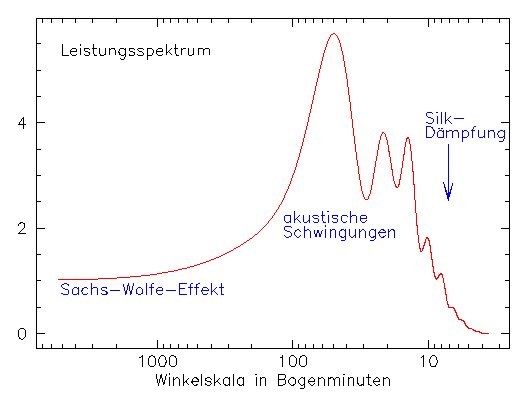
\includegraphics[scale=1]{pow}
\caption{Mögliches Leistungsspektrum des CMB. Auf der Abzisse ist die Winkelskala in Bogenminuten angegeben -- alternativ wird hier auch oft Ordnung des Multipols angegeben. Die Ordinate ist in willkürlichen Einheiten angegeben. Quelle: \cite{A+R}}
\label{pow}
\end{figure}
Die unterschiedlichen Ursachen der primären Anisotropie tragen auf unterschiedlich großen räumlichen Skalen zum CMB bei.
Hat man nun die Anisotropien des CMB gemessen und von Vordergrundquellen und sekundären Effekten bereinigt, betrachtet man die Stärke der Anisotopien in Abhängigkeit von ihrer räumlichen Größe.
Dies klingt nach einer typischen Aufgabe für eine Fouriertransformation, da jedoch der von uns aus beobachtete CMB eine Kugeloberfläche darstellt, ist es nötig das Signal nicht in trigonometrische Funktionen, sondern in Kugelflächenfunktionen zu zerlegen.\cite{Schneider}\cite{S+W00} Die mathematischen Grundlagen sind jedoch dieselben. 
Man kann sich dies auch wie folgt vorstellen:
Man wählt zwei Punkte in festem Abstand $r$, misst ihre Temperatur und bestimmt ihre relative Temperaturdifferenz:
\begin{equation}
\Delta T = \frac{|T_1-T_2|}{\langle T\rangle }
\end{equation}
wobei $\langle T\rangle$ die durchschnittliche Temperatur des CMB ist. Man berechnet dies für alle Punktpaare mit dem festen Abstand $r$ und mittelt über diese. Man erhält so den Wert des sogenannten Leistungspektrums $C(r)$ für den Wert $r$ und kann dies für alle Punktabstände wiederholen, um das Leistungsspektrum als Funktion des Abstands $r$ zu erhalten.\cite{Schneider} In der Praxis betrachtet man das Leistungsspektrum nicht in Abhängigkeit vom Punktabstand, sondern von der Ordnung $l$ der Kugelflächenfunktionen, also $C_l$. $C_0$ stellt dabei die mittlere Temperatur dar, $C_1$ die Stärke der dipolen Temperaturdifferenz, usw.
Dabei arbeitet man meist mit $l\left(l+1\right)C_l$, als Funktion über $l$. Alternativ kann anstatt $l$ auch eine Winkelskala verwendet werden, ein derartiges Leistungsspektrum ist in Abbildung \ref{pow} abgebildet.

Das aufgrund der obigen Effekte vorhergesagte und inzwischen auch gemessene Leistungsspektrum besteht dabei primär aus drei Teilen:
\begin{itemize}
\item Bei großen Skalen dominiert der Sachs-Wolfe-Effekt.\cite{A+R} Groß bedeutet hierbei deutlich größer als die Horizontlänge zum Zeitpunkt der Rekombination. Die Horizontlänge gibt an, welche Distanz zwei Punkte maximal haben könnten, damit sie bei endlicher Lichtgeschwindigkeit $c$ seit dem Urknall je in einem kausalem Zugsamenhang stehen konnten. Sie beträgt laut Peter Schneider\cite{Schneider} für ein flaches Universum etwa:
\[ \theta_{H,rec} \approx 1,8^\circ \]
\item Auf Winkelskalen $\ll\theta_{H,rec}$ betrachtet man Gebiete, welche vor der Rekombination innerhalb des Horizonts lagen, also miteinander gewechselwirkt haben können. Hier kommt es zu den sogenannten Akustischen Schwingungen:
Das heiße Baryonen-Photonen-Gemisch besaß einen Druck, der bestrebt war, der Schwerkraft entgegenzuwirken. Zog sich eine überdichte Materiewolke unter dem Einfluss der Schwerkraft zusammen, so presste der Druck des Baryonen-Photonen-Gemischs sie wieder auseinander, bis erneut die Schwerkraft überwog und sich das Gebiet wieder zusammenzog, und so fort. Durch das Entgegenwirken von Schwerkraft und Druck kam es also zu Schwingungen im kosmischen Gemisch.
Zu derartigen Schwingungen kann es natürlich nur kommen, wenn die Materiewolke kleiner als die Horizontlänge ist. Konkret muss die Wolke klein genug sein, dass die Druckwellen genügend Zeit haben um von einem Ende der Gaswolke zum anderen Ende zu kommen -- ansonsten baut sich der Druck nicht schnell genug auf um das Kollabieren aufzuhalten und die Wolke stürzt, ohne zu Schwingen, in sich zusammen.\cite{S+W00} Das Gemisch aus Baryonen und Photonen lässt sich als eine relativistische Flüssigkeit betrachten und hat somit eine Schallgeschwindigkeit von $c_s\approx\sqrt{P/\rho}\approx c/\sqrt{3}$.\cite{Schneider} Man bezeichnet die daraus folgende maximale Ausdehnung als Schallhorizont, er unterscheidet sich aufgrund der hohen Schallgeschwindigkeit nur durch einen Faktor $1/\sqrt3$ von der oben definierten Horizontlänge.
Aufgrund des endlichen Alters des Universums und der Endlichkeit der Lichtgeschwindigkeit fangen die Wolken je nach Größe unterschiedlich früh an zu schwingen, also sind die Schwingungen gleich großer Materiewolken synchronisiert. Ist eine Materiewolke also klein genug um zu schwingen, so schwingt sie phasengleich mit anderen Wolken gleicher Größe. Zum Zeitpunkt der Rekombination sind also alle gleichgroßen Materiewolken in der gleichen Schwingungsphase.\cite{A+R} Dadurch könnten wir die Schwingungen deutlich im Leistungsspektrum sehen. Da es sich um Dichtewellen handelt, nennt man sie Akustische Schwingungen; ein anderer, physikalisch nicht ganz korrekter Name für die Peaks der Schwingungen ist Doppler-Peaks.\cite{S+W00}
\item Solange die Rekombination nicht abgeschlossen ist, also noch elektrisch geladene Teilchen im kosmischen Gemisch enthalten sind, wechselwirken die Photonen mit dem kosmischen Gas. Dadurch treiben die entstehenden Materiewolken auseinander, sofern sie nicht massereich genug sind. Kleine Dichteschwankungen werden also weggedämpft, man bezeichnet diesen Effekt nach seinem Entdecker als Silk-Dämpfung (engl. Silk-Damping).\cite{A+R} Dazu kommt noch ein weiterer Effekt: Die Rekombination geschah nicht exakt instantan, sondern dauerte eine gewisse Zeit. Die Photonen des CMB kommen zu uns also aus einer Schale endlicher Dicke. Betrachten wir nun einen Punkt im CMB, so beobachten wir die mittlere Temperatur über eine kleine Strecke entlang der Sichtlinie durch die Schale. Ist die Winkelskala, auf der wir die Anisotropien beobachten, kleiner als die Dicke der Schale, so befinden sich mehrere Maxima und Minima innerhalb der Schalendicke, wodurch die Fluktuationen weggemittelt werden. Dieser Effekt wirkt auf den gleichen Skalen wie die Silk-Dämpfung. Durch diese Effekte werden auf Skalen $\lesssim 5'$ d.h. $l\gtrsim2500$ die Temperaturfluktuationen stark gedämpft und fallen rasch ab.\cite{Schneider}
\end{itemize}

\section{Kosmologische Parameter im CMB}
\begin{figure}[tbhp]
\center
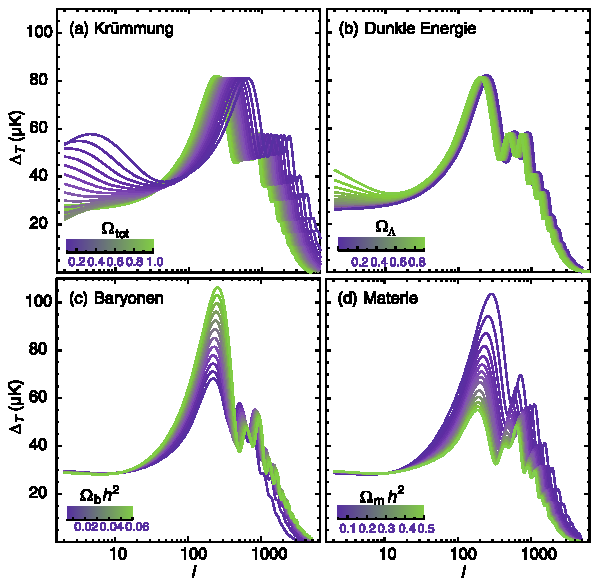
\includegraphics[scale=0.8]{cmbvar}
\caption{Vorhersage des Leistungsspektrum des Kosmischen Hintergrunds bei Variation der Materiedichten. In allen Fällen ist das Referenzmodell beschrieben durch $\Omega_m + \Omega_\Lambda = 1$, $\Omega_\Lambda = 0.65$, $\Omega_b h^2 = 0.02$, $\Omega_m h^2 = 0.147$ und einer Steigung des primordialen Dichtespektrums n = 1, entsprechend dem Harrison–Zeldovich-Spektrum. Quelle: \cite{Schneider}}
\label{cmbvar}
\end{figure}
Die genaue Form des aus den besprochenen Effekten berechneten Leistungspektrums -- also die Stärke und Lage der Maxima und Minima, ihre Abstände zueinander sowie die Stärke der Silk-Dämpfung und des Sachs-Wolfe-Effekts -- hängen teils äußerst empfindlich von den kosmologischen Parametern ab. Vermisst man also den Mikrowellenhintergrund äußerst präzise, so kann man aus dem Leistungsspektrum praktisch alle kosmologischen Parameter äußerst präzise bestimmen -- also insbesondere:
\begin{itemize}
\item Der Dichteparameter der Baryonischen Materie $\Omega_b$
\item der Dichteparameter der heißen dunklen Materie $\Omega_{HDM}$
\item der Dichteparameter der Materie $\Omega_m=\Omega_b+\Omega_{HDM}$
\item der Dichteparameter der Dunklen Energie $\Omega_\Lambda$
\item der gesamte Dichteparameter $\Omega_{tot}=\Omega_m+\Omega_\Lambda$ und damit den Krümmungsparameter $k$
\item der heutige Wert des Hubbleparamters $H_0$
\item die Normierung $\sigma_8$
\item und der Formparameter des Leistungsspektrums $\Gamma$.\cite{Schneider}
\end{itemize}
Wir wollen an den folgenden Beispielen verdeutlichen, wie man diese aus dem Leistungsspektrum bestimmen kann. Abbildung \ref{cmbvar} zeigt die Abhängigkeit von einigen der Parametern, besonders empfehlenswert sind auch die Animationen unter \url{http://space.mit.edu/home/tegmark/movies.html}.

Die Stärke und die Frequenz der akustischen Schwingungen wird durch die Stärke der Rückstellkraft, also des Drucks, bestimmt. Dieser hängt wiederum von der Zusammensetzung des kosmischen Gemisches ab.\cite{S+W00}

Die größten Materiewolken, die noch zu schwingen begonnen haben, hatten eine Ausdehnung, die der Schallhorizontlänge entspricht. Daher definiert der Schallhorizont den Grundton des Mikrowellenhintergrunds, also die Lage des ersten Dopplerpeaks. Da wir den Zeitpunkt der Rekombination und die Schallgeschwindigkeit kennen, können wir die Schallhorizontlänge berechnen. Die berechnete Länge ist mit der Lage des ersten Maximums durch die Krümmung des Raumes verknüpft, denn eine bekannte Länge erscheint aus einer bekannten Entfernung unter einem unterschiedlich großem Winkel, je nachdem, ob und wie stark der Raum gekrümmt ist. In einem positiv gekrümmten (sphärischen) Raum erscheint er unter einem größerem Winkel, als in einem negativ gekrümmten (hyperbolischen) Raum. Durch exaktes Vermessen der Lage des ersten Maximums lässt sich also die Krümmung des Universums bestimmen. Diese ist außerdem direkt mit $\Omega_{tot}$ verknüpft.\cite{S+W03}

\section{Erforschung der Anisotropien}\label{Missionen}
\begin{figure}
\center
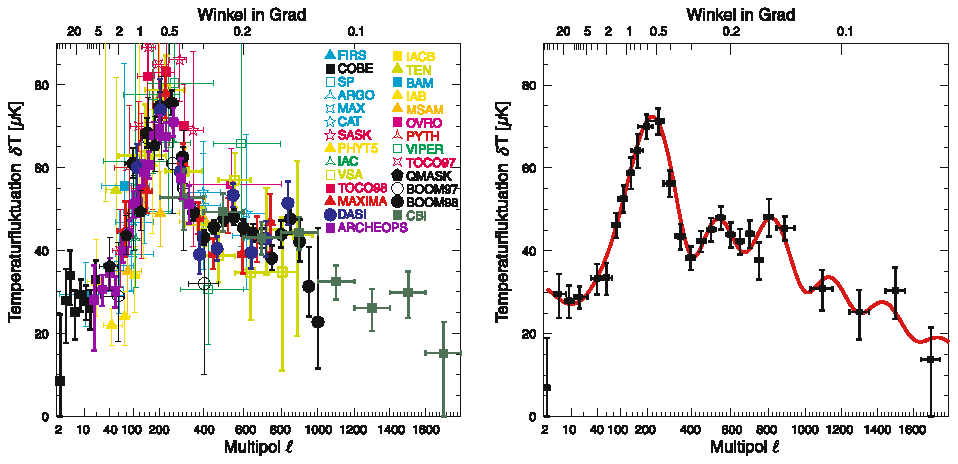
\includegraphics[scale=1]{mess}
\caption{Die Messwerte der CMB-Anisotropien auf dem Stand von Ende 2002. Links die einzelnen Werte, rechts die gewichteten Mittel und das dazu am besten passende Spektrum. Quelle: \cite{Schneider}}
\label{mess}
\end{figure}

\begin{figure}
\center
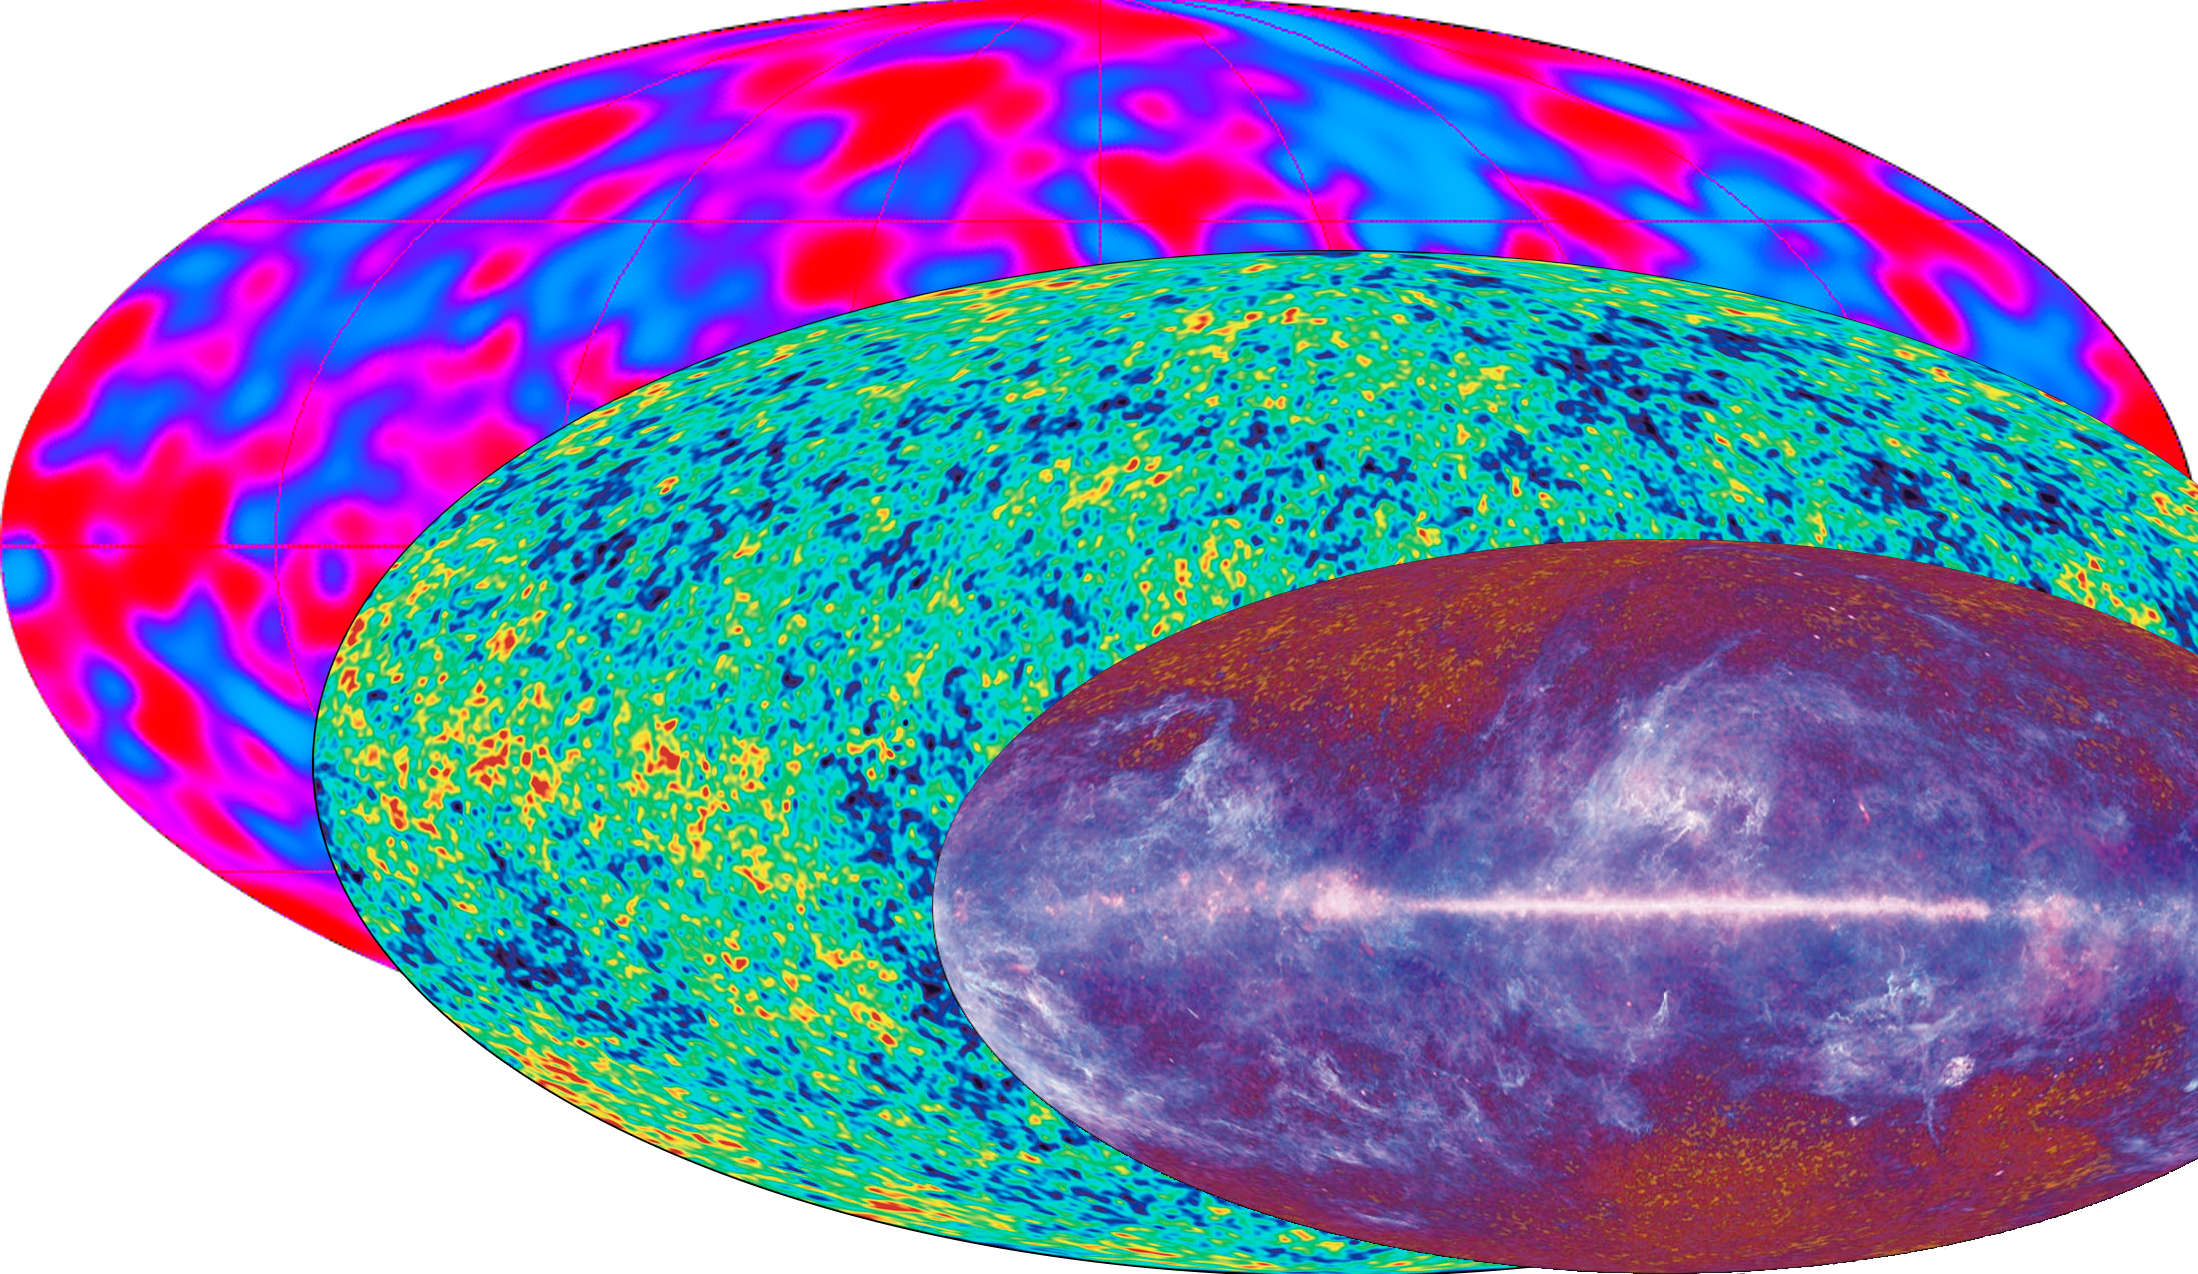
\includegraphics[scale=0.15]{CMB}
\caption{Vergleich der Karten von COBE, WMAP und Plank (von hinten). Bei der Karte von Planck wurden die Vordergrundobjekte bisher noch nicht herausgerechnet.}
\label{cmb}
\end{figure}

Nach COBE wurden zahlreiche weitere Missionen gestartet, um den CMB genauer zu vermessen, darunter auch zwei weitere Satelliten: WMAP und Plank.
Satelliten sind sind wie bei den meisten Wellenlängen auch bei Mikrowellenteleskopen von Vorteil, da die Atmosphäre Strahlung absorbiert und somit das Bild trübt. Darüber hinaus können sie den kompletten Himmel abmustern und somit 360\degree Ansichten aufnehmen. Die Auflösung eines Teleskops hängt allgemein von der Öffnung des Teleskops und der Wellenlänge der zu detektierenden Strahlung ab. Da die Größe von Satelliten technisch stark begrenzt ist, können sie nicht die selbe Auflösung wie ein bodengestütztes Teleskop erreichen. Aufgrund der großen Wellenlänge der Hintergrundstrahlung ist die Auflösung von Mikrowellenteleskopen ohnehin relativ gering.

Die vielen anderen Experimente wurden entweder mit Ballonen in der Stratosphäre oder zumindest an kalten und/oder hochgelegenen Orten wie dem Südpol durchgeführt, da dort die Effekte der Atmosphäre schwächer sind. Sie haben den Vorteil einer vergleichsweise hohen Winkelauflösung.

Die 1989 gestartete Sonde COBE hatte eine Winkelauflösung von nur sieben Grad (420 Bogenminuten) und war somit nicht in der Lage die akustischen Schwingungen zu detektieren!\cite{S+W00} Um die damals noch unsichere Existenz der akustischen Schwingungen nachzuweisen und damit die kosmologischen Parameter zu bestimmen, wurden verschiedene erdgebundene Missionen gestartet. Den Ballon-Experimenten BOOMERanG und MAXIMA, sowie dem am Südpol stationiertem Projekt Dasi gelang unabhängig voneinander, den ersten Dopplerpeak genau und den zweiten ansatzweise zu vermessen.\cite{S+W03} Um die Genauigkeit der Vermessung des Leistungsspektrums zu erhöhen, musste man nun erneut Satellitenmissionen starten, da Land- und Ballonexperimente durch ihr begrenztes Sichtfeld beziehungsweise durch ihre begrenzte Flugdauer nur einen kleinen Teil des Himmels aufnehmen können.
Der Satellit WMAP (früher: MAP oder auch Explorer 80) kartografierte von 2001 bis 2010 den CMB mit einer Winkelauflösung von 53 bis 13 Bodenminuten.\cite{PJ1} Er maß auf den Frequenzen 22, 30, 40, 60 und 90 GHz.
Die europäische Nachfolgemission, der Satellit Planck, wurde 2009 ins Weltall geschossen und beobachtete dort bis Anfang 2012 mit zwei Geräten auf neun verschieden Frequenzen zwischen 25 und 1000 GHz, seit dem planmäßigen Zuendegehen des Kühlmittels am 16. Januar 2012 kann nur noch das \glqq Low Frequency Instrument\grqq (LFI) weiter-betrieben werden\cite{PJ1}\cite{pm}.
Planck konnte anstatt der vorgesehenen zwei sogar fünf komplette Himmelsdurchmusterungen aufnehmen und hatte dabei Winkelauflösungen von bis zu 4 Bogenminuten. % und kann damit …
Dank der neun verschiedenen Frequenzen kann Planck Vordergrundquellen besser eliminieren. Die Auswertung der Daten wird Anfang 2013 fertig sein und unsere kosmologischen Weltmodelle entweder mit hoher Genauigkeit bestätigen oder neue Fragen aufwerfen.

\newpage
\bibliography{lit}{}
\bibliographystyle{unsrtdin}

\end{document}
